\begin{figure}[h]
\begin{center}
\begin{adjustbox}{width=\textwidth}

% Gradient Info
  
\tikzset {_2yn49zl61/.code = {\pgfsetadditionalshadetransform{ \pgftransformshift{\pgfpoint{0 bp } { 0 bp }  }  \pgftransformrotate{0 }  \pgftransformscale{2 }  }}}
\pgfdeclarehorizontalshading{_f0h1xn2np}{150bp}{rgb(0bp)=(0.88,0.88,0.88);
rgb(37.5bp)=(0.88,0.88,0.88);
rgb(49.53571319580078bp)=(0.88,0.88,0.88);
rgb(62.5bp)=(1,0,0);
rgb(100bp)=(1,0,0)}
\tikzset{_ao557rzfs/.code = {\pgfsetadditionalshadetransform{\pgftransformshift{\pgfpoint{0 bp } { 0 bp }  }  \pgftransformrotate{0 }  \pgftransformscale{2 } }}}
\pgfdeclarehorizontalshading{_b1qqyoil7} {150bp} {color(0bp)=(transparent!61);
color(37.5bp)=(transparent!61);
color(49.53571319580078bp)=(transparent!75);
color(62.5bp)=(transparent!75);
color(100bp)=(transparent!75) } 
\pgfdeclarefading{_gj5ns3oqm}{\tikz \fill[shading=_b1qqyoil7,_ao557rzfs] (0,0) rectangle (50bp,50bp); } 

% Gradient Info
  
\tikzset {_5ocf120kv/.code = {\pgfsetadditionalshadetransform{ \pgftransformshift{\pgfpoint{0 bp } { 0 bp }  }  \pgftransformrotate{0 }  \pgftransformscale{2 }  }}}
\pgfdeclarehorizontalshading{_25n4qjk0b}{150bp}{rgb(0bp)=(1,0,0);
rgb(37.5bp)=(1,0,0);
rgb(62.5bp)=(0,0,1);
rgb(100bp)=(0,0,1)}
\tikzset{_m8uedxkdp/.code = {\pgfsetadditionalshadetransform{\pgftransformshift{\pgfpoint{0 bp } { 0 bp }  }  \pgftransformrotate{0 }  \pgftransformscale{2 } }}}
\pgfdeclarehorizontalshading{_49t70h8cn} {150bp} {color(0bp)=(transparent!75);
color(37.5bp)=(transparent!75);
color(62.5bp)=(transparent!75);
color(100bp)=(transparent!75) } 
\pgfdeclarefading{_ugfmlo9rg}{\tikz \fill[shading=_49t70h8cn,_m8uedxkdp] (0,0) rectangle (50bp,50bp); } 

% Gradient Info
  
\tikzset {_daocnbh0q/.code = {\pgfsetadditionalshadetransform{ \pgftransformshift{\pgfpoint{0 bp } { 0 bp }  }  \pgftransformrotate{0 }  \pgftransformscale{2 }  }}}
\pgfdeclarehorizontalshading{_03e54ezl1}{150bp}{rgb(0bp)=(0,0,1);
rgb(37.5bp)=(0,0,1);
rgb(62.5bp)=(0,0,1);
rgb(100bp)=(0,0,1)}
\tikzset{_48is8yhe5/.code = {\pgfsetadditionalshadetransform{\pgftransformshift{\pgfpoint{0 bp } { 0 bp }  }  \pgftransformrotate{0 }  \pgftransformscale{2 } }}}
\pgfdeclarehorizontalshading{_w9dk1nw55} {150bp} {color(0bp)=(transparent!75);
color(37.5bp)=(transparent!75);
color(62.5bp)=(transparent!50);
color(100bp)=(transparent!50) } 
\pgfdeclarefading{_thlshpcj1}{\tikz \fill[shading=_w9dk1nw55,_48is8yhe5] (0,0) rectangle (50bp,50bp); } 

% Gradient Info
  
\tikzset {_2e7ef02nx/.code = {\pgfsetadditionalshadetransform{ \pgftransformshift{\pgfpoint{0 bp } { 0 bp }  }  \pgftransformrotate{0 }  \pgftransformscale{2 }  }}}
\pgfdeclarehorizontalshading{_qf8n4pbxh}{150bp}{rgb(0bp)=(1,0,0);
rgb(37.5bp)=(1,0,0);
rgb(62.5bp)=(0.03,0,1);
rgb(100bp)=(0.03,0,1)}
\tikzset{_i6071vu9t/.code = {\pgfsetadditionalshadetransform{\pgftransformshift{\pgfpoint{0 bp } { 0 bp }  }  \pgftransformrotate{0 }  \pgftransformscale{2 } }}}
\pgfdeclarehorizontalshading{_mpfm3gyjm} {150bp} {color(0bp)=(transparent!75);
color(37.5bp)=(transparent!75);
color(62.5bp)=(transparent!75);
color(100bp)=(transparent!75) } 
\pgfdeclarefading{_a3543rpu3}{\tikz \fill[shading=_mpfm3gyjm,_i6071vu9t] (0,0) rectangle (50bp,50bp); } 
\tikzset{every picture/.style={line width=0.75pt}} %set default line width to 0.75pt        

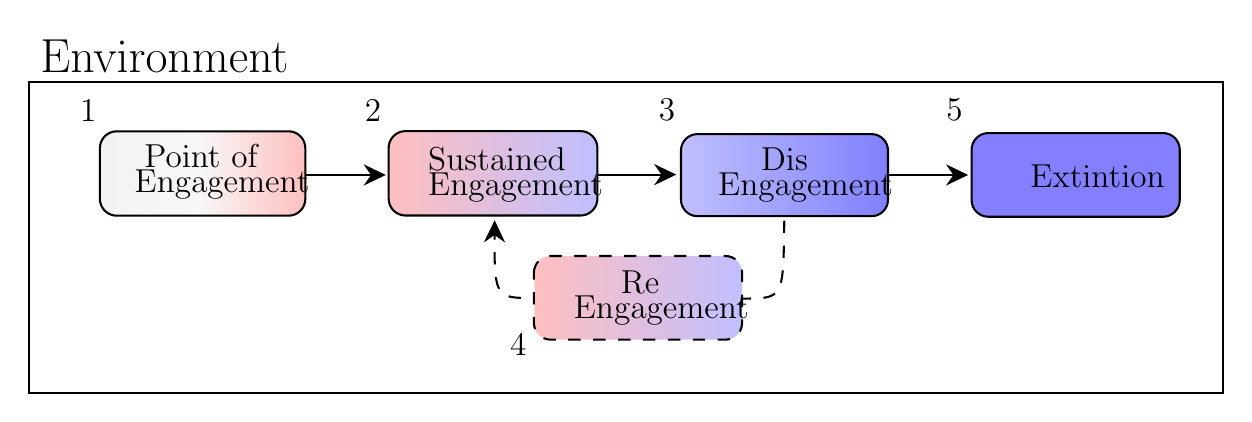
\begin{tikzpicture}[x=0.75pt,y=0.75pt,yscale=-1,xscale=1]
%uncomment if require: \path (0,200); %set diagram left start at 0, and has height of 200

%Shape: Rectangle [id:dp21453085870796063] 
\draw   (14.1,36.6) -- (589.6,36.6) -- (589.6,186.3) -- (14.1,186.3) -- cycle ;
%Rounded Rect [id:dp8669331486657136] 
\path  [shading=_f0h1xn2np,_2yn49zl61,path fading= _gj5ns3oqm ,fading transform={xshift=2}] (48.4,68.36) .. controls (48.4,63.87) and (52.04,60.22) .. (56.53,60.22) -- (139.24,60.22) .. controls (143.73,60.22) and (147.37,63.87) .. (147.37,68.36) -- (147.37,92.76) .. controls (147.37,97.25) and (143.73,100.89) .. (139.24,100.89) -- (56.53,100.89) .. controls (52.04,100.89) and (48.4,97.25) .. (48.4,92.76) -- cycle ; % for fading 
 \draw   (48.4,68.36) .. controls (48.4,63.87) and (52.04,60.22) .. (56.53,60.22) -- (139.24,60.22) .. controls (143.73,60.22) and (147.37,63.87) .. (147.37,68.36) -- (147.37,92.76) .. controls (147.37,97.25) and (143.73,100.89) .. (139.24,100.89) -- (56.53,100.89) .. controls (52.04,100.89) and (48.4,97.25) .. (48.4,92.76) -- cycle ; % for border 

%Straight Lines [id:da4505594811913791] 
\draw    (147.6,81.26) -- (183.16,81.26) ;
\draw [shift={(186.16,81.26)}, rotate = 180] [fill={rgb, 255:red, 0; green, 0; blue, 0 }  ][line width=0.08]  [draw opacity=0] (10.72,-5.15) -- (0,0) -- (10.72,5.15) -- (7.12,0) -- cycle    ;
%Rounded Rect [id:dp29846373438871854] 
\path  [shading=_25n4qjk0b,_5ocf120kv,path fading= _ugfmlo9rg ,fading transform={xshift=2}] (187.51,68.26) .. controls (187.51,63.77) and (191.16,60.13) .. (195.65,60.13) -- (279.95,60.13) .. controls (284.44,60.13) and (288.09,63.77) .. (288.09,68.26) -- (288.09,92.66) .. controls (288.09,97.15) and (284.44,100.8) .. (279.95,100.8) -- (195.65,100.8) .. controls (191.16,100.8) and (187.51,97.15) .. (187.51,92.66) -- cycle ; % for fading 
 \draw   (187.51,68.26) .. controls (187.51,63.77) and (191.16,60.13) .. (195.65,60.13) -- (279.95,60.13) .. controls (284.44,60.13) and (288.09,63.77) .. (288.09,68.26) -- (288.09,92.66) .. controls (288.09,97.15) and (284.44,100.8) .. (279.95,100.8) -- (195.65,100.8) .. controls (191.16,100.8) and (187.51,97.15) .. (187.51,92.66) -- cycle ; % for border 

%Straight Lines [id:da4495263911578298] 
\draw    (288.09,81.1) -- (323.09,81.1) ;
\draw [shift={(326.09,81.1)}, rotate = 180] [fill={rgb, 255:red, 0; green, 0; blue, 0 }  ][line width=0.08]  [draw opacity=0] (10.72,-5.15) -- (0,0) -- (10.72,5.15) -- (7.12,0) -- cycle    ;
%Rounded Rect [id:dp9135925108190124] 
\path  [shading=_03e54ezl1,_daocnbh0q,path fading= _thlshpcj1 ,fading transform={xshift=2}] (328.37,69.49) .. controls (328.37,65.13) and (331.91,61.59) .. (336.28,61.59) -- (420.18,61.59) .. controls (424.55,61.59) and (428.09,65.13) .. (428.09,69.49) -- (428.09,93.21) .. controls (428.09,97.58) and (424.55,101.11) .. (420.18,101.11) -- (336.28,101.11) .. controls (331.91,101.11) and (328.37,97.58) .. (328.37,93.21) -- cycle ; % for fading 
 \draw   (328.37,69.49) .. controls (328.37,65.13) and (331.91,61.59) .. (336.28,61.59) -- (420.18,61.59) .. controls (424.55,61.59) and (428.09,65.13) .. (428.09,69.49) -- (428.09,93.21) .. controls (428.09,97.58) and (424.55,101.11) .. (420.18,101.11) -- (336.28,101.11) .. controls (331.91,101.11) and (328.37,97.58) .. (328.37,93.21) -- cycle ; % for border 

%Rounded Rect [id:dp630049377495355] 
\path  [shading=_qf8n4pbxh,_2e7ef02nx,path fading= _a3543rpu3 ,fading transform={xshift=2}] (257.51,128.36) .. controls (257.51,123.9) and (261.13,120.29) .. (265.58,120.29) -- (349.73,120.29) .. controls (354.19,120.29) and (357.8,123.9) .. (357.8,128.36) -- (357.8,152.55) .. controls (357.8,157.01) and (354.19,160.62) .. (349.73,160.62) -- (265.58,160.62) .. controls (261.13,160.62) and (257.51,157.01) .. (257.51,152.55) -- cycle ; % for fading 
 \draw  [dash pattern={on 4.5pt off 4.5pt}] (257.51,128.36) .. controls (257.51,123.9) and (261.13,120.29) .. (265.58,120.29) -- (349.73,120.29) .. controls (354.19,120.29) and (357.8,123.9) .. (357.8,128.36) -- (357.8,152.55) .. controls (357.8,157.01) and (354.19,160.62) .. (349.73,160.62) -- (265.58,160.62) .. controls (261.13,160.62) and (257.51,157.01) .. (257.51,152.55) -- cycle ; % for border 

%Straight Lines [id:da1505945863891579] 
\draw    (427.92,81.26) -- (463.72,81.26) ;
\draw [shift={(466.72,81.26)}, rotate = 180] [fill={rgb, 255:red, 0; green, 0; blue, 0 }  ][line width=0.08]  [draw opacity=0] (10.72,-5.15) -- (0,0) -- (10.72,5.15) -- (7.12,0) -- cycle    ;
%Rounded Rect [id:dp7652426478992563] 
\draw  [fill={rgb, 255:red, 8; green, 0; blue, 255 }  ,fill opacity=0.5 ] (468.37,69.13) .. controls (468.37,64.68) and (471.98,61.07) .. (476.44,61.07) -- (560.59,61.07) .. controls (565.05,61.07) and (568.66,64.68) .. (568.66,69.13) -- (568.66,93.33) .. controls (568.66,97.79) and (565.05,101.4) .. (560.59,101.4) -- (476.44,101.4) .. controls (471.98,101.4) and (468.37,97.79) .. (468.37,93.33) -- cycle ;
%Curve Lines [id:da6295563644706698] 
\draw  [dash pattern={on 4.5pt off 4.5pt}]  (238.57,106.4) .. controls (238.32,140.92) and (238.67,140.53) .. (257.51,140.53) ;
\draw [shift={(238.6,103.1)}, rotate = 90.44] [fill={rgb, 255:red, 0; green, 0; blue, 0 }  ][line width=0.08]  [draw opacity=0] (10.72,-5.15) -- (0,0) -- (10.72,5.15) -- (7.12,0) -- cycle    ;
%Curve Lines [id:da022545744318036687] 
\draw  [dash pattern={on 4.5pt off 4.5pt}]  (378.14,103.27) .. controls (377.57,140.99) and (378.09,140.81) .. (357.8,140.81) ;

% Text Node
\draw (65.5,23.28) node  [font=\fontsize{0.67em}{0.8em}\selectfont] [align=left] {\begin{minipage}[lt]{68.75pt}\setlength\topsep{0pt}
\begin{center}
{\LARGE Environment}
\end{center}

\end{minipage}};
% Text Node
\draw (97.09,79.56) node  [font=\fontsize{0.67em}{0.8em}\selectfont] [align=left] {\begin{minipage}[lt]{47.87pt}\setlength\topsep{0pt}
\begin{center}
{\large Point of}\\{\large Engagement}
\end{center}

\end{minipage}};
% Text Node
\draw (238.5,80.46) node  [font=\fontsize{0.67em}{0.8em}\selectfont] [align=left] {\begin{minipage}[lt]{47.87pt}\setlength\topsep{0pt}
\begin{center}
{\large Sustained}\\{\large Engagement}
\end{center}

\end{minipage}};
% Text Node
\draw (378.23,81.35) node  [font=\fontsize{0.67em}{0.8em}\selectfont] [align=left] {\begin{minipage}[lt]{47.87pt}\setlength\topsep{0pt}
\begin{center}
{\large Dis}\\{\large Engagement}
\end{center}

\end{minipage}};
% Text Node
\draw (518.51,81.23) node  [font=\fontsize{0.67em}{0.8em}\selectfont] [align=left] {\begin{minipage}[lt]{32.64pt}\setlength\topsep{0pt}
\begin{center}
{\large Extintion}
\end{center}

\end{minipage}};
% Text Node
\draw (308.67,140.46) node  [font=\fontsize{0.67em}{0.8em}\selectfont] [align=left] {\begin{minipage}[lt]{47.87pt}\setlength\topsep{0pt}
\begin{center}
{\large Re}\\{\large Engagement}
\end{center}

\end{minipage}};
% Text Node
\draw (37.33,43.67) node [anchor=north west][inner sep=0.75pt]   [align=left] {{\large 1}};
% Text Node
\draw (174.53,43.67) node [anchor=north west][inner sep=0.75pt]   [align=left] {{\large 2}};
% Text Node
\draw (316.2,43) node [anchor=north west][inner sep=0.75pt]   [align=left] {{\large 3}};
% Text Node
\draw (244.53,156.67) node [anchor=north west][inner sep=0.75pt]   [align=left] {{\large 4}};
% Text Node
\draw (454.73,43) node [anchor=north west][inner sep=0.75pt]   [align=left] {{\large 5}};

\end{tikzpicture}

\end{adjustbox}
\end{center}
\caption{\textbf{Diagram summarizing the different stages of the negagement process mode}.  Solid and dashed lines represent compulsory and  optional paths. Moving from the left to the right we can imagine 1 as being the first interaction that an individual has with an object. This might happen as the result of a prior belief that the object is able to provide a pleasurable experience. The individual will interact with the object for as long as this last one is able to provide a gratifying experience(i.e. 2). However, if this is not the case, or constraints from the surrounding environment emerge, the individual will gradually reduce their interaction with the object (i.e. 3). At this point we can either observe an alternation between re-engagement and disengagement (i.e. 4) or reach an inevitable state of complete withdrawal from the object (i.e. 5)}
\label{fig: eng_proc_model_1}
\end{figure}